\chapter{\hlc[red]{EVDT Framework}} \label{ch:evdt}

Computational models have been closely linked to the pursuit of sustainable development and with its definition, stemming from the World3 system dynamics model underlying the Club of Rome's \textit{The Limits to Growth} report in 1972 \cite{meadowsLimitsGrowth1972}.

"Sustainable Development involves not just one but four complex interacting systems. It deals with a global economy...; it focuses on social interactions...; it analyzes the changes in complex Earth systems...; and it studies the problems of governance". \cite{sachsAgeSustainableDevelopment2015} [Compare this to the EVDT framework]

We are far from the first to argue that such integration is necessary, nor to recognize that it is easier said than done \cite{shahumyanIntegrationLandUse2017}.

There have been many land use and transportation models. The open source UrbanSim, for example, combines land use, transportation, and certain environmental factors in a dynamic, area-based simulation system that, similar to \ac{evdt}, is a collection multiple models \cite{waddellUrbanSimModelingUrban2002}.

The agent-based \ac{ilute} model simulated the urban spatial form, demographics, travel behavior, and environmental impacts for the Toronto area \cite{millerHistoricalValidationIntegrated2011}.

Existing \ac{pss} have often been criticized for being lacking with regard to "visioning, storytelling sketching, and developing strategies," as well as being "too generic, too complex, inflexible, incompatible..., oriented towards technology rather than problems" \cite{brommelstroetPlanningSupportSystems2010}" This leads to what some have called the "implementation gap" of \acp{pss} \cite{BottlenecksBlockingWidespread}.

For the past couple of decades, there has been a recognition that \acp{dss} and \acp{pss} must include more than purely spatial analysis components \cite{geertmanPlanningSupportSystems2004}.

The closest attempt to what we are proposing is probably that of Shahumyan and Moeckel, though their approach focused on linking together existing models in a loose manner using ArcGIS Model Builder, to avoid having to gain access to proprietary source code. While their example focused on combinging transportation, land use, mobile emissions, building emissions, and land cover, with only limited feedbacks, their approach could be extended to capture the full feedback loops proposed by \ac{evdt}. Their example is also proof that the kind of loose integration of library of models that \ac{evdt} envisions is possible \cite{shahumyanIntegrationLandUse2017}. 

Lauf et al. combined cellular automata with systems dynamics to capture both spatial dynamics and macroscale demand-supply dynamics in order to simulate residential development \cite{laufUncoveringLanduseDynamics2012}

Pert et al. combined environmental and decision-making in a participatory model to improve conservation outcomes \cite{pertParticipatoryDevelopmentNew2013}. 

Miller argues that, despite the historical dificulties that integrated urban models have had, there is reason to be optimistic about the state of the art moving forward, particularly for integrating transportation and land-use models in particular \cite{millerIntegratedUrbanModeling2018}. <---important to discuss at more length

Is not itself a means of planning and implementing projects. It is not a full life-cycle tool such as \ac{ppbs} \cite{hatryCriteriaEvaluationPlanning1972}

Clifton et al. breaks down the various ways of modeling the urban form into five categories (though they do not assert that these are comprehensive or mutually exclusive), as seen in Table \ref{table:urban_form} \cite{cliftonQuantitativeAnalysisUrban2008}. While \ac{evdt} does not focus specifically on urban form, it is interested in these types of models, with the case studies presented in this work focusing on landscape ecology and community design in particular. One downside of examinations of urban form is that they tend to focus on areas and residences, while various forms of social exclusion are better measured by focusing on individuals instead \cite{scottRoleUrbanForm2008}.

\begin{table}[h]
%\begin{center}
\small
\caption[Five categories of urban form models]{Five categories of urban form models. Adapted from \cite{cliftonQuantitativeAnalysisUrban2008}}
\label{table:urban_form}
\makebox[\linewidth]{
\begin{tabular}{ L{2.5cm} L{2.5cm}  L{2.5cm} L{2.5cm} L{2.5cm} L{2.5cm}} \hline
Perspective & Principal concern & Disciplinary Orientation & Scale & Nature of Data & Common Metrics  \\ \hline

Landscape ecology & Environmental protection & Natural scientists & Regional & Land cover & Land cover change; Contagion \\ 

Economic structure & Economic efficiency & Economists & Metropolitan & Employment and population & Density gradient; Land value  \\

Transportation planning & Accessibility & Transportation planners & Submetropolitan & Employment, population and transportation network & Expected travel time; capacity  \\

Community design & Social welfare & Land-use planners & Neighborhood & Local \ac{gis} data & Proximity to needs; Zoning; Accessibility \\

Urban design & Aesthetics and walkability & Urban designers & Block face & Images, surveys, and audits & Lot size; Accessibility \\ \hline

\end{tabular}
}
%\end{center}
\end{table}


The motivation for combining so many variables from different disciplines stems from both push and pull factors. The push factors are the simple increase in availability of data, as has already been described, along with the increase in the interoperability of the variables (which the work described in this thesis is trying to help contribute to). The primary pull factor is our increased understanding of - and appreciation for - the complex relationships between these domains, relationships that were previously ignored in analyses \cite{gaheganMultivariateGeovisualization2007}. 


Position \ac{evdt} using the different dimensions of models proposed in \cite{harrisQuantitativeModelsUrban1972}:

\begin{enumerate}[itemsep=0pt,parsep=0pt]
	\item{descriptive vs. analytic}
	\item{holistic vs. partial}
	\item{macro vs. micro}
	\item{static vs. dynamic}
	\item{deterministic vs. probabilistic}
	\item{simultaneous vs. sequential (directly calculate the output or go through intermediate phases)}
\end{enumerate}

Goodchild defines six different \ac{gis} data field model types and states that "no current \ac{gis} gives its users full access to all six":

\begin{enumerate}
    \setlength{\itemsep}{0pt}%
    \setlength{\parskip}{0pt}%
	\item{Sample randomly located points (e.g. weather stations, \ac{lidar} data)}
	\item{Sample randomly from a grid of regularly space points (e.g. many data validation studies}
	\item{Divide the area into a grid in which each rectangular cell records the average, total, or dominant value; i.e. raster data (e.g. satellite imagery)}
	\item{Divide the area into homogenous regions and record the average, total, or dominant value in each area (e.g. census data, soil maps)}
	\item{Record the locations of lines of fixed values (e.g. contour or isopleth maps}
	\item{Divide the area into irregular shaped triangles and assume the field varies linearly within each (e.g. some \acp{dem})}
\end{enumerate}

In the mid 90s, \ac{gis} had several limitations \cite{goodchildGeographicInformationSystems1994}:

\begin{itemize}
    \setlength{\itemsep}{0pt}%
    \setlength{\parskip}{0pt}%
	\item{Two-dimensional, with some excursions into three}
	\item{Static, with some limited support for time dependence}
	\item{Limited capabilities for representing forms of interaction between objects}
	\item{A diverse and confusing set of data models}
	\item{Dominated by the map metaphor}
\end{itemize}

To some extent, many of these issues, such as the lack of three dimensional systems, persisted well past the 90s \cite{goodchildTwentyYearsProgress2010}.

Yamu et al. argue that urban modeling should treat the urban form as a \ac{cas} and use fractal metrics to develop scenarios for planning purposes \cite{yamuAssumingItAll2016}.

In order for cost-benefit analysis to maximize economic welfare, the following conditions must be met \cite{krutillaWelfareAspectsBenefitCost1961}:

\begin{enumerate}[itemsep=0pt,parsep=0pt]
	\item{Opportunity costs are borne by beneficiaries in  such wise as to retain the initial income distribution}
	\item{The initial income distribution is in some sense "best}
	\item{The marginal social rates of transformation between any two commodities are everywhere equal to their corresponding rates of substitution except for the area(s) justifying the intervention in question}
\end{enumerate}

More details modeling, as well as breaking down specific costs and benefits (as opposed to converting them to monetary terms and summing them) and attributing them to specific goals, can circumvent these constraints, though at the cost of increased complexity \cite{hillGoalsAchievementMatrixEvaluating1972}.

The Law of requisite variety from the field of cybernetics says that the variety (the number of elements or states) of the control device must be at least equal to that of the disturbances \cite{ashbyRequisiteVarietyIts1991}. Any development plan is going to fall far short of the variety expressed by human society and the natural environment. Planning efforts must then make reliance on the natural homeostasis behavior of such systems and of more flexible, ad hoc measures not specified in the plan in order to make up the difference in variety. \cite{mcloughlinSystemGuidanceControl1972}

\section{\hlc[yellow]{The Framework}} 

The \ac{evdt} Framework is process for developing a \ac{dss} for a sustainable development application. This processed is characterized by five basic elements: 

\begin{enumerate}
	\item{The use of systems architecture \& stakeholder analysis to identify needs, design the \ac{dss}, and understand the context through the use of the \ac{saf}. This requires significant engagement with as many of the stakeholders as is feasible (if not more).}
	\item{Collaborative development of the \ac{dss} that continues that stakeholder engagement.}
	\item{A concept of the sustainable development application as a complex \ac{sets}, typically involving the Environment, Human Vulnerability and Societal Impact, Human Behavior and Decision-Making, and Technology Design. This concept undergirds the \ac{dss} architecture and is critical as it provides the capability both for detailed technical analysis as well as feeding back into the design of data collection systems . \label{item:evdt}}
	\item{An interactive \ac{dss}. This can take the form of an in-browser page, a standalone application for a computer or phone, or even a tabletop exercise with paper documents.}
	\item{A consideration towards modularity and re-use in future applications. This includes both technical components of the \ac{dss} product and broader capacity building in the community.}
\end{enumerate}

Each of these elements span the entire lifecycle of an \ac{evdt} project, but can still be usefully considered in the order listed.

\subsection{\hlc[yellow]{System Architecture Framework}} \label{sec:saf}

The first element of the \ac{evdt} Framework builds upon Maier's \cite{maierArtSystemsArchitecting2009} and Crawley's \cite{crawley2004} work to apply systems architecture to international collaborations \cite{pfotenhauerArchitectingComplexInternational2016} and sustainable development \cite{ovienmhadaInclusiveDesignEarth2021}. As defined by Maier, systems architecture the art and science of creating and building complex systems, and in particular that part of systems development most conerned with scoping, structuring, and certification \cite{maierArtSystemsArchitecting2009}. This tends to refer to the high level form and function of a system, rather than detailed design. Other's, such as Crawley prefer to characterize it as the mapping of function to form such that the essential features of the system are represented. The intent of architecture is to reduce ambiguity, employ creativity, and manage complexity \cite{crawleySystemArchitectureStrategy2015}. Arguably this is a more specific formulation of Maier's definition. In general, Space Enabled and I tend to use Crawley's definition, both due to its clarity, and for the various qualitative and quantitative methods that have been developed to work well with this formulation. The \ac{saf}, as adapted by Space Enabled and previous applied in sustainable development applications \cite{ovienmhadaInclusiveDesignEarth2021}, involves six steps, shown in Figure \ref{fig:saf}. It seeks to center the full network of stakeholders and invite them into a collaborative development process. By stakeholders, I mean the people, organizations, and communities that either influence the design and operation of the system or are impacted by the system. 

\begin{figure}[t] 
\centering
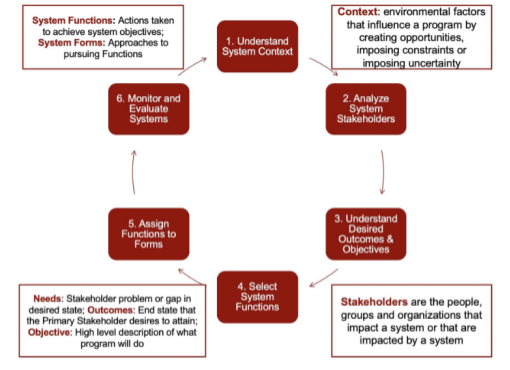
\includegraphics[width=0.9\textwidth]{Figures/chap3/SAF.png}
\caption[Six steps of SAF]{Six steps of \ac{saf}.}
\label{fig:saf}
\end{figure}

Each of these steps is amenable to, and arguably requires, collaborative participation from stakeholders, linking this methodology to \ac{pgis}. Such an approach means that the primary benefits of systems architecture (listed below) \cite{crawley2004} do not just accrue to central authorities or technocrats, but are held by the community themselves.

\begin{enumerate}[itemsep=0pt,parsep=0pt]
	\item{Architecture is a way to understand complex systems.}
	\item{Architecture is a way to design complex systems}
	\item{Architecture is a way to design standards and protocols to guide the evolution of long-lived systems.}
	\item{Architecture is a way to manage complex systems.}
\end{enumerate}

The stakeholders are involved in defining the system, understanding the System Context (the external factors that influence and constrain the system), identify System Objectives (the high level description of what the program will do), and develop the System Functions (the specific actions taken to achieve the objectives) and System Forms (the approaches and structures used to pursue the functions). 

Notably unlike some forms of stakeholder analysis that primarily use stakeholder input to inform system requirements at the beginning of the development cycle, \ac{saf} seeks to involve the stakeholders in ongoing monitoring, evaluation, and participation. Multiple techniques are available for coordinating input and involvement from various stakeholders, with varying levels of detail, time requirements, and balance of quantitative versus qualitative information. Examples include multi-stakeholder tradespace exploration \cite{fitzgeraldRecommendationsFramingMultistakeholder2016}, multicriteria negotiations \cite{sparrevikUseMulticriteriaInvolvement2011}, and collaborative sketch planning \cite{vonkSociotechnicalPSSDevelopment2010}.


\subsection{\hlc[yellow]{Collaborative Development}} 

Involving stakeholders in the development process, in addition to the requirements definition process, is key for ensuring adoption and capacity building. This has been recognized by the \ac{pgis} movement, which increasingly emphasizes the importance of open source software \cite{williamsonTheirworkDevelopmentSustainable2011, dodgeMappingModesMethods2011}. It is also core to the Data Action framework which, responding to the idea that "data is never raw, it's collected," emphasizes the use of participatory and collaborative methods for collecting and using data \cite{williamsDataActionUsing2020}. Collaborative development is increasingly feasible as barriers have dropped over the past couple of decades. Knowledge and familiarity with computers and programs has expanded, access to sufficient hardware is increasingly common (particularly with the rise of cloud computing platforms), and both synchronous and asynchronous online collaboration tools have proliferated. Obviously such barriers have not been universally eliminated. Furthermore, even in the absence of barriers, not everyone desires to be a computer programmer, earth scientist, \ac{eo} specialist, or social scientist, even part-time. Collaborative development must therefore take different forms in each project, being as welcome as possible to all while accommodating stakeholder preferences and constraints.

\subsection{\hlc[cyan]{EVDT Questions \& Models}} 

The \ac{evdt} Framework conceptualizes the application system from two different perspectives. The first is the system boundaries and stakeholders perspective from \ac{saf} shown in Figure \ref{fig:saf}. The second perspective focuses on combining the established fields of sociotechnical systems \cite{rouseUnderstandingChangeComplex2012,siddiqiSociotechnicalSystemsSustainability2017,sussmanTeachingComplexSociotechnical2010} and socio-environmental systems \cite{elsawahEightGrandChallenges2020} into \ac{sets}. To accomplish this, at least four components are considered: the Environment (data including Landsat, Sentinel, VIIRs, in-situ environmental data and knowledge, etc.); Human Vulnerability and Societal Impact (data including census and survey-based demographic data, eocsystem services valuations, NASA's Socioeconomic Data and Applications Center, local knowledge of impacts, etc.); Human Behavior and Decision-Making (data including policy histories, mobility data, urban nightlight data, community input, etc.); and Technology Design for earth observation systems including satellites, airborne platforms and in-situ sensors (data including design parameter vectors for such systems). The data from each of these domains is used by established models in each domain, which are adapted to work in concert to address the needs identified during the stakeholder analysis. These four components, shown in Figure \ref{fig:model}, seek to encapsulate the major interacting aspects of sustainable development and consider them from a \ac{sets} perspective. 

We are far from the first to argue that such integration is necessary, nor to recognize that it is easier said than done. The closest attempt to what is proposed here is probably that of Shahumyan and Moeckel, though their approach focused on linking together existing models in a loose manner using ArcGIS Model Builder, to avoid having to gain access to proprietary source code. While their example focused on combining transportation, land use, mobile emissions, building emissions, and land cover, with only limited feedbacks, their approach could be extended to capture the full feedback loops proposed by \ac{evdt}. Their example is also proof that the kind of loose integration of library of models that \ac{evdt} envisions is possible \cite{shahumyanIntegrationLandUse2017}. 

The motivation for combining so many variables from different disciplines stems from both push and pull factors. The push factors are the simple increase in availability of data, along with the increase in the interoperability of the variables (which this work itself is trying to contribute to). The primary pull factor is our increased understanding of - and appreciation for - the complex relationships between these domains, relationships that were previously ignored in analyses \cite{gaheganMultivariateGeovisualization2007}. 

\begin{figure}[h]
    \centering
    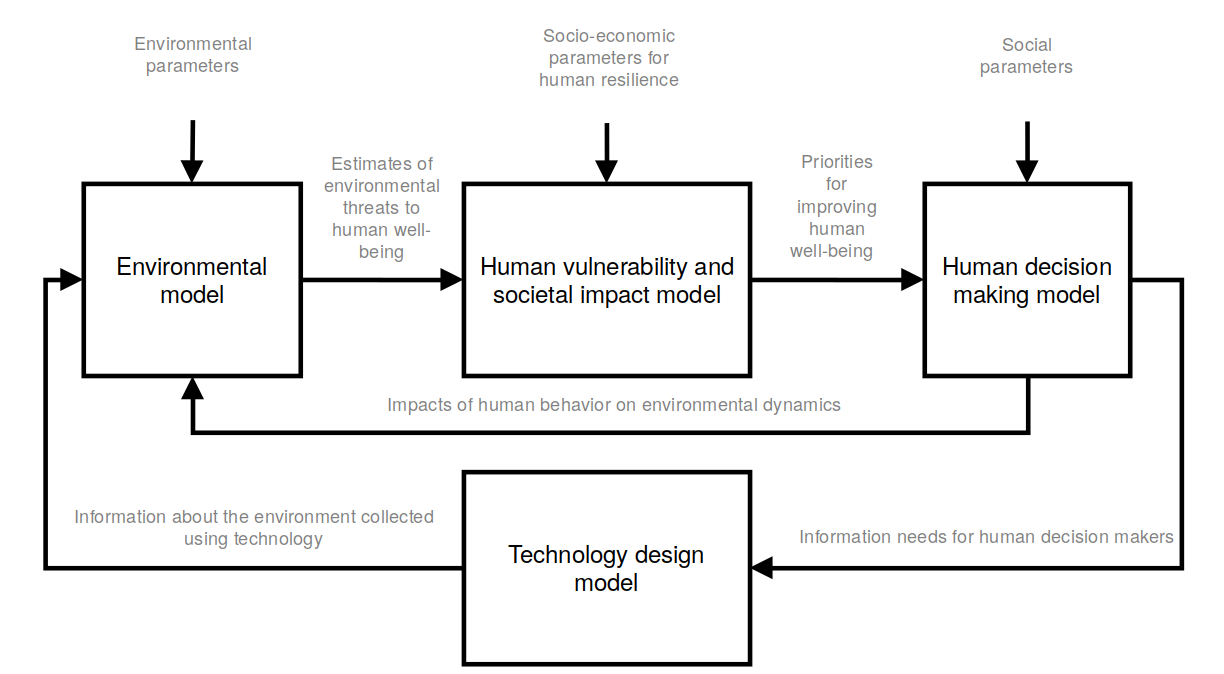
\includegraphics[scale=0.3]{Figures/chap3/modelflow.png}
    \caption[Generic version of EVDT Model] {Generic version of the Environment - Vulnerability - Decision - Technology Model}
    \label{fig:model}
\end{figure}

This set of four models with the particular linkages shown in Figure \ref{fig:model} are not the only form that \ac{evdt} can take, merely the most general arrangement. Some applications may involve replacing a model with a human-in-the-loop (e.g. having the user themself substitute for the decision-making model) or omitting a model altogether. For other applications, it may make sense to conceptually break a model into two or more components. In the Vida project, it was considered worthwhile to separate the social impact model into two components, one focusing on public health (the obvious priority when dealing with COVID-19) and one focusing on non-health metrics (such as income, employment, etc.). Such a separation can be useful if either significantly different modeling methodologies are going to be used or if the linkages with the other \ac{evdt} components are different from one another. 

One way to determine the optimal arrangment of \ac{evdt} components is to consider what questions the user or researcher is seeking to answer with this application of \ac{evdt}. For instance, the default \ac{evdt} arrangement shown in Figure \ref{fig:model} was motivated primarily by the following four questions:

\begin{enumerate} \setlength{\itemsep}{0pt} \setlength{\parskip}{0pt}
    \item What is happening in the natural environment?
    \item How will humans be impacted by what is happening in the natural environment?
    \item What decisions are humans making in response to environmental factors and why?
    \item What technology system can be designed to provide high quality information that supports human decision making?
\end{enumerate}

Alternate questions may result in a different configuration or set of components (further discussion of this in Section \ref{sec:intended}). The point of \ac{evdt} is not to insist upon a particular set of linkages and feedbacks, but rather to encourage a consideration of such linkages between domains in general, and to consider them through a systems engineering perspective. Of course answering the structuring questions, and even phrasing them in the first place, requires the use of collaborations.

\subsection{\hlc[yellow]{Interactive Decision Support System}} 

A key aspect of the term \ac{dss} is the word "support." Crawley et al. state that the goal of a \ac{dss} is to "\emph{enhance} the efficiency of decision makers by providing tools to quantitatively and qualitatively explore a space of alternatives for single or multiple decisions" [emphasis added] \cite{crawleySystemArchitectureStrategy2015}. This means that the \ac{evdt}-developed \ac{dss} should not present decisions as a \textit{fait accompli} but instead support stakeholders in developing their own solutions. Ideally this means that individual stakeholders can directly handle and explore any simulations or models used, along with their underlying assumptions and structure. If this is not feasible, an indirect form of interaction can be used, such as when a stakeholder provides verbal instruction to someone who then implements that instruction in the \ac{dss}. The latter option can be quite useful when there are barriers of language, familiarity, or technical knowledge, and is commonly used in purposeful gaming \cite{rossGamebasedLearningSystems2014}, wargaming \cite{hansonImprovingOperationalWargaming2016,selvaRevitalizingWargamingNecessary15,shlapakReinforcingDeterrenceNATO2016}, and role playing gaming \cite{groganStrategicEngineeringGaming2012,groganFederatedSimulationGaming2012}. Additionally, in contrast to Crawley's definition which centers on the "efficiency of decision-makers," we argue that an ideal \ac{dss} should cause a decision-maker to consider multiple perspectives (such as the four models of \ac{evdt} and those of other stakeholders) and thereby make \textit{better} decisions as well.

\subsection{\hlc[yellow]{Re-use \& Community Development}} 

One of the key motivations of participatory, stakeholder-involved processes is capacity building. In the case of the \ac{evdt} Framework, this includes both capacity building in a specific application community and in the broader practitioner community of those using \ac{eo}, \ac{gis}, and systems engineering for sustainable development. To that end, the \ac{dss} should be designed with re-use and modularity in mind. The ability to track mangrove health in Brazil \cite{reidInteractiveModelAssessing2020} proved to be useful in a later application in Indonesia \cite{lombardoEnvironmentVulnerabilityDecisionTechnologyFrameworkDecision2022}. A key aspect of this is making as much of the \ac{dss} code available in open source repositories.

The second form of capacity building is pursued by developing a community of practice around \ac{evdt} and related endeavors.

\section{\hlc[cyan]{Intended Applications \& User Types}} \label{sec:intended}

\ac{evdt} is not intended to be an exclusive project of Space Enabled. It also not intended to be a framework used by isolated individuals. We actively invite involvement from other systems engineers and those from other disciplines. Through this proposed thesis and other related projects, the framework will be refined, initial applications demonstrated, a basis of code built (already available online \cite{bluerasterBlueRasterVida2021,reidEVDTRepository2020,reidMITVidaRepository2021}), and a community of collaboration sprouted. These will can be built upon for building a community of practice, where individuals can contribute in a variety of ways, as shown in Figure \ref{fig:development}.

\begin{figure}[h]
	\centering
	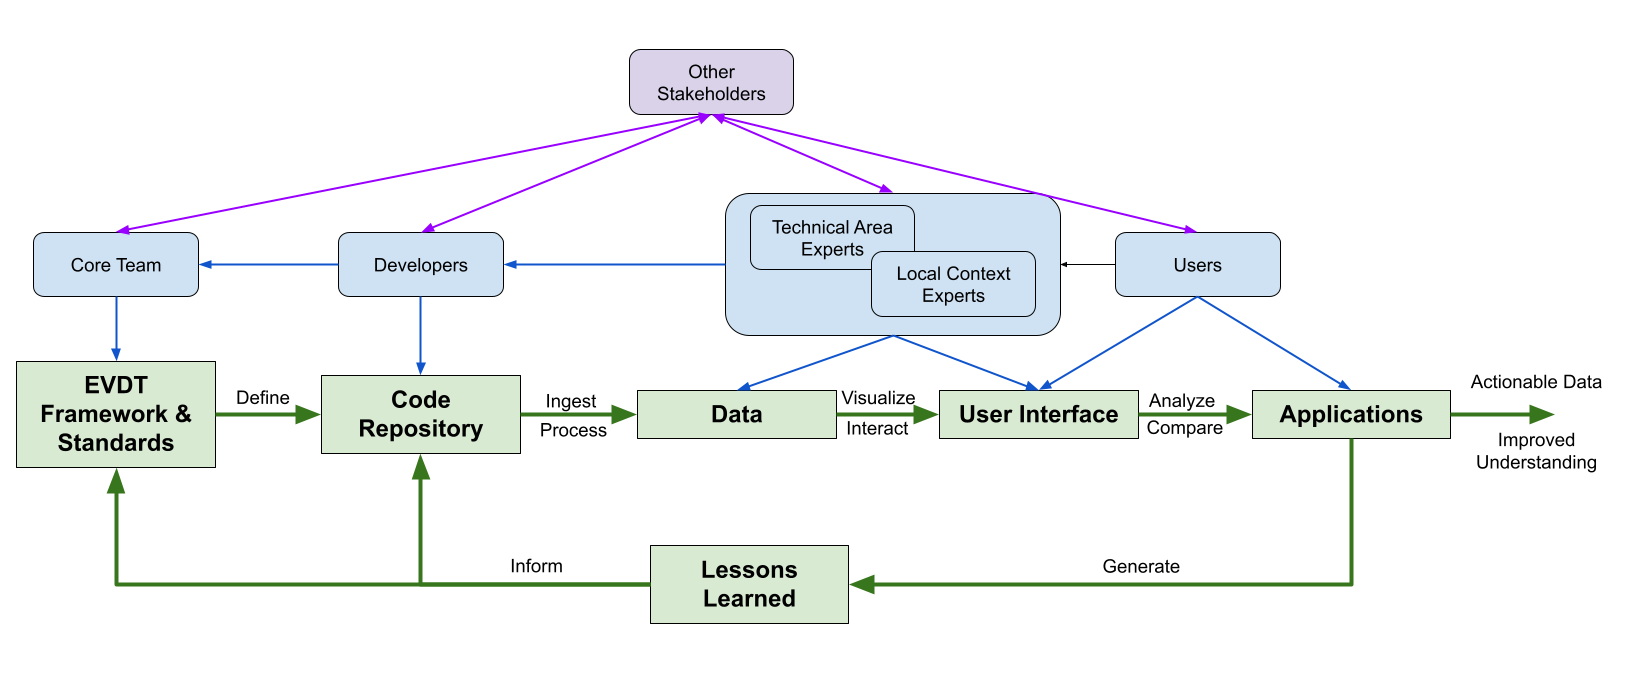
\includegraphics[scale=0.25]{Figures/chap3/Graphic_2_Development.png}
	\caption[The EVDT development pipeline] {The EVDT development pipeline. Note that the different community groups, shown in blue, are not necessarily discrete and one individual could simultaneously participate in multiple.}
	\label{fig:development}
\end{figure}

It is worth further describing some of the categories of \ac{evdt} community members shown in the blue boxes of Figure \ref{fig:development}. What follows will be a generalized discussion of these categories. Specific instances for this thesis are discussed in Chapters \ref{ch:mangroves} and \ref{ch:vida}.

Moving from left to right, the \textit{Core Team} refers to those directly involved in the development of the \ac{evdt} Framework. Right now this is essentially a set of researchers in Space Enabled and some close academic affiliates. This team is likely to remain predominently academic moving forward, though could transition to involving individuals or organizations from \acp{ngo} in the future. The members of this team will typically have expertise with sustainable development and \acp{dss}, significant experience with \ac{evdt}, and investment in its success. Particularly once \ac{evdt} is more developed, this core team is likely to be formally defined.

The \textit{Developers} includes all those who actively develop the models, user interfaces, visualizations, and other associated aspects of the \ac{dss} software for the various \ac{evdt} projects. These will typically be individuals with expertise in \ac{gis}, coding, and/or data processing. Thus they are likely to work in academia or as analysts in a government agency or \ac{ngo}, though the project will be open source, membership in this category will not be formally defined and participation will be encouraged at any level of expertise or degree of involvement. Currently the Developer team is largely the same as the Core Team, though we have some developer involvement from other collaborators as well.

\textit{Technical Area Experts} refers to experts in some relevant domain to an \ac{evdt} project but are consulted but not directly involved in the ongoing development of the \ac{evdt} Framework and code repository. This could include individuals such as ecosystem services economists, human mobility researchers, or fisheries experts. They will typically come from the ranks of academia, though it is not unreasonable to expect some number of government analysts or \ac{ngo} researchers.

\textit{Local Context Experts} refers to those who have a high level of knowledge of the \ac{sets} and stakeholders of a particular \ac{evdt} project. This could include a local community leader, an experienced activist, or a local government official. This category is grouped together with \textit{Technical Area Experts} as the line between the two is oftentimes blurry. A local university researcher who studies the economics of informal housing and who specializes in the city involved with a particular \ac{evdt} project is arguably both a Technical Area Expert and a Local Context Expert.

\textit{Users} refers to those who directly use the \ac{dss} software developed through an \ac{evdt} project. Exactly who these are will depend on the specific project and thus their level of experience with mapping, earth science, or development may vary significantly. They should be direct stakeholders in the specific \ac{evdt} project and have some involvement with the decision-making process (though not necessarily formal involvement). 

It should also be emphasized that while Figure \ref{fig:development} is fairly linear, the \ac{evdt} Framework emphasizes collaborative development. One person may serve multiple roles in the pipeline and, even if not, stakeholders, including users, should be involved throughout the \ac{dss} development process.

As the number of applications increase and the code is refined, the various models used in the applications may themselves be the first members of an openly accessible library of models. Potential user groups could adapt and reuse \ac{evdt} components in other applications, without having to start from scratch. Initially this would likely still require significant code expertise, but it is entirely possible for functionality to be created to allow for `plug-and-play.' A user may be able to, in browser or on desktop, select a geographic area of interest (e.g. the Sóc Trăng Province of Vietnam), select an environmental model (e.g. coastal forest health), a societal impact model (e.g. cyclone vulnerability), a decision-making model (land use conversion and conservation policy), and a technology model (satellite versus in-situ monitoring), all without writing a line of code (though perhaps being required to import new datasets themselves). Such functionality, along with the recruitment pipeline shown in Figure \ref{fig:development}, help to expand participation in all aspects of \ac{evdt}. In this way the user base will be expanded beyond initially invested experts.

We are cognizant that making \ac{evdt} truly participatory is easier said than done, but we do believe it is a worthy goal. In addition to model interoperability standardization, the code moderators will need to specify accessibility norms as well, so as to ensure usability by individuals with a wide range of backgrounds. Existing prototypes have made some steps in this direction, by having multiple language options available. Thus far, this has been accomplished by existing language knowledge of code moderators as well as the occasional volunteer translator, but some more targeted efforts may be required in the future to specifically recruit translators for targeted languages.

Language is not the only accessibility barrier, however. Terminology, presentation, and interactiveness can also be differentiately accessible to different individuals, depending factors such as educational or cultural background. That said, these difficulties can be addressed via some of the same methods that are already core to the \ac{evdt} methodology: namely partnerships with local collaborators; stakeholder analysis; and iterative, participative design. 

Another consideration in the future of \ac{evdt} are the types of applications that it will be used for. Some potential applications include:

\begin{enumerate} \setlength{\itemsep}{0pt} \setlength{\parskip}{0pt}
    \item To inform sustainable development policies. Ex) Comparing the impact of different conservation and zoning policies on the local environment and on economic outcomes.  \label{item:policy}
    \item To educate on the connections between the different \ac{evdt} domains. Ex) Demonstrating the local ecosystem services value of treecover in an urban environment.
	\item To facilitate the comparison of different remote sensing data products for particular applications. Ex) Considering whether to commission periodic aerial surveys of an area or to rely on "free" civil satellite data, such as Landsat and Sentinel. \label{item:data}.
    \item To facilitate the exploration and evaluation of new sensing technology architectures for particular applications. Ex) Designing a new \ac{lidar} satellite to assist forest management in a particular region. \label{item:tech}
    \item To facilitate scientific research on ecosystem services and/or the impacts of human behavior on the environment. Ex) Simulating different casual connections and comparing the simulated data with historical data, to assess the strength of those connections.
    \item To provide a basis for studies of the effectiveness of different \ac{dss} attributes. Ex) Assessing visualization techniques, workshop formats, etc. \label{item:user}
\end{enumerate}

These applications are varying levels of interest and importance to different stakeholders, and some could potentially be viewed as competing for development resources and focus. In some cases they may rely upon different configurations of the \ac{evdt} components, as shown in Figure \ref{fig:combo}. For instance Items \ref{item:data} and \ref{item:tech} (best served by configuration B of Figure \ref{fig:combo}) require a functional model of the relationships between different remote observation design parameters and performance parameters, along with a means of visualizing and exploring the tradespace (as has been proposed by Siddiqi et al. \cite{siddiqiValuingNewEarth2019}). A user who is predominantly interested in Item \ref{item:policy} (configuration A) may find this functionality irrelevant or outright distracting.

On the other hand, some applications are more complementary. While the Item \ref{item:policy} is likely to be a government official or community member while the Item \ref{item:user} user is likely to be an academic researcher, the findings from Item \ref{item:user} would result in the design of \ac{evdt} being improved, so as better serve the needs of the Item \ref{item:policy} user.

Ideally, \ac{evdt} would be open to all these applications and more. In practice, care must be taken so that interests of one user group do not unintentionally dominate those of others or, worse, that the interests of the developers do not send them on a path counter to the interests of the users. This will thus require ongoing discussion and consideration with the \ac{evdt} community.

It should also be recognized that not all users will engage with the \ac{evdt} \ac{dss} software products directly or in the same way. As shown in Figure \ref{fig:development}, some stakeholders and community members will participate in the \ac{saf} process, but may not directly interact with the \ac{evdt} software products themselves. This is both due to the fact that many people are unlikely to have the time or inclination to do so (understandably so) and due to various barriers that will doubtlessly remain despite the efforts of \ac{evdt} developers. Such barriers include access to the internet, computing power, and electricity. While all of these are becoming available to an increasing number of people globally, they are by no means ubiquitous. Initial prototypes have \ac{evdt} have pursued both offline, desktop version and online, browser-based versions to try and accomodate different levels of resource access. Such issues will need to be considered as part of future development decisions as well.

Finally, this envisioned development and expansion process is fundamentally a "snowball model." Existing team members collaborate with new partners and their communities. This results in additional team members who can then collaborate with others. \ac{evdt} may (and should aim) to one day be easily accessible even in the absence of connections to existing community members, but that is not in the immediate future.

\clearpage
\begin{figure}[h]
	\centering
	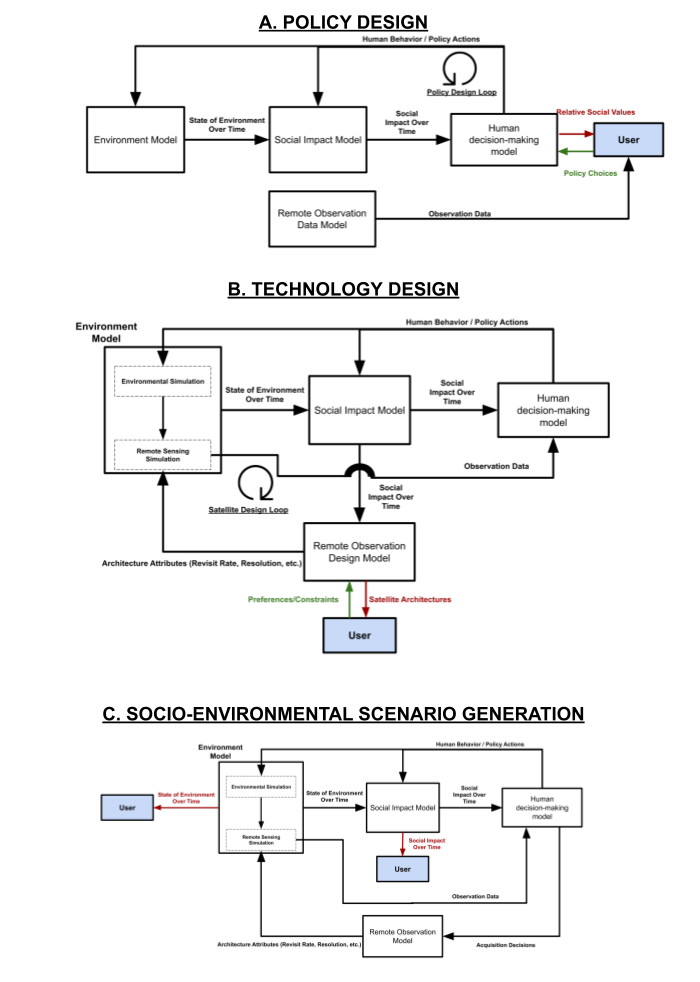
\includegraphics[scale=0.5]{Figures/chap3/Loops_Combined.png}
	\caption{Three example EVDT research configurations}
	\label{fig:combo}
\end{figure}
\clearpage

\section{\hlc[cyan]{Novelty}}

It is important to establish what aspects of \ac{evdt} are novel and how this framework relates to the current state of practice. 

Computational models have long been closely linked to the pursuit of sustainable development and with its definition, stemming from the World3 system dynamics model underlying the Club of Rome's \textit{The Limits to Growth} report in 1972 \cite{meadowsLimitsGrowth1972}. As was discussed in Section \ref{sec:se}, the development field would largely come to repudiate such efforts in the mid-to-late 1970s, only to come back around to modeling on their own terms in the subsequent decades. Thus it cannot be said that \ac{evdt} is new in saying that modeling plays an important role in sustainable development. 

Nor can it be said that \ac{evdt} is the first to advance the concept of multidisciplinary, integrated models in development applications. To refer to just a handful of examples:

\begin{itemize} \setlength{\itemsep}{0pt} \setlength{\parskip}{0pt}
	\item{The open source UrbanSim combines land use, transportation, and certain environmental factors in a dynamic, area-based simulation system that, similar to \ac{evdt}, is a collection of multiple models \cite{waddellUrbanSimModelingUrban2002}.}
	\item{The agent-based \ac{ilute} model simulated the urban spatial form, demographics, travel behavior, and environmental impacts for the Toronto area \cite{millerHistoricalValidationIntegrated2011}.}
	\item{The TripEnergy model combines an environmental submodel (transportation systems) and societal impact submodel (energy consumption and emissions of vehicles) \cite{needellEfficientlySimulatingPersonal2018}. It is then combined with a model of human decision-making to create Tripod, "a smartphone-based system to influence individual real-time travel decisions by offering information and incentives to optimize system-wide energy performance" \cite{azevedoTripodSustainableTravel2018}.}
	\item{The closest attempt to what we are proposing here is probably that of Shahumyan and Moeckel, though their approach focused on linking together existing models in a loose manner using ArcGIS Model Builder, to avoid having to gain access to proprietary source code. While their example focused on combinging transportation, land use, mobile emissions, building emissions, and land cover, with only limited feedbacks, their approach could be extended to capture the full feedback loops proposed in \ac{evdt}. Their example is also proof that the kind of loose integration of library of models that \ac{evdt} envisions is possible \cite{shahumyanIntegrationLandUse2017}.}
\end{itemize} 

In the field of earth science, integrated models have also become increasingly common. Originally developed for operational weather forecasting, \acp{osse} have found widespread use for designing earth observation systems at \ac{nasa} and elsewhere \cite{masutaniObservingSystemSimulation2010}, by linking models of environmental phenomena with simulations of observing platforms (both hypothetical and real). These models are rigorously validated \cite{erricoDevelopmentValidationObservingsystem2013} and are often custom-made for a particular mission. Significant progress has been made however by the  Hydrological Sciences Laboratory and Earth Science Technology Office at \ac{nasa} in developing the \ac{lis}, a more reusable and inter-operable modeling tool with numerous earth sciences applications (soil moisture, hydrology, meteorology, etc.) \cite{kumarMissionSimulationEvaluation2015}. One of these uses is the easier development of \acp{osse}, as a means of facilitating technological development. Since the development of the \ac{lis}, the Hydrological Sciences Laboratory has worked to make the earth science models more accurate, utilize  a broader range of computational methods, and standardize the validation and evaluation processes for \acp{osse}.

Systems engineering has also recently seen a handful of approaches proposed for use in sustainable development. In 2020, Honoré-Livermore et al. sought to address the \acp{sdg} in arctic coastal regions via an approach grounded in \ac{ses} and the \ac{spade} methodology \cite{honore-livermoreAddressingSustainableDevelopment2020}. The \ac{spade} methodology was developed specifically for sustainable development applications. The five components of its name constitute five non-linear steps, each of which has various specific associated methodologies \cite{haskinsSystemsEngineeringAnalyzed2008}, as shown in Figure 3.

\begin{figure}[h]
\centering
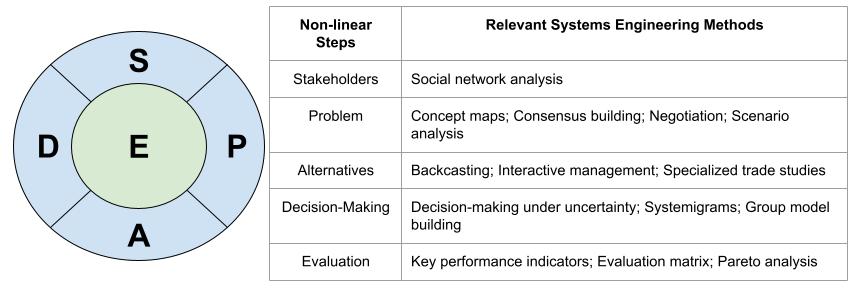
\includegraphics[scale=0.4]{Figures/chap3/spade.png}
\caption[The SPADE Methodology and associated methods]{The Stakeholders-Problem-Alternatives-Decision-Making-Evaluation (SPADE) Methodology and associated methods. Adapted from Haskins, 2008 \cite{haskinsSystemsEngineeringAnalyzed2008} as seen in \cite{reidSystemsEngineeringAppliedPendingPublication}.}
\label{fig:spade}
\end{figure}

Van Zyl and Root meanwhile used a transdisciplinary approach involving Wilbur's integral systems theory \cite{esbjorn-hargensOverviewIntegralTheory2010} and the \ac{catwoe} framework from \ac{ssm} \cite{checklandSoftSystemsMethodology2000} to design sustainable agricultural principles in New Zealand \cite{vanzylTransdisciplinaryDesignImplementation2020}.

Other recent approaches focus on scenario planning and education for understanding evolution of the urban form \cite{geyerSystemsEngineeringMethodology2014}, sustainable land-use planning that relies upon multilevel stakeholder partnerships \cite{puchol-salortUrbanPlanningSustainability2021}, a synthesis of participatory planning with systems engineering for sustainable regional planning \cite{aspenDevelopingParticipatoryPlanning2021}, and leveraging human-centered design to address the \acp{sdg} \cite{muellerUsingHumanCenteredDesign2020}. A survey of sustainable development applications of systems engineering can be found in Yang and Cormican, 2021 \cite{yangCrossoversConnectivitySystems2021}, which itself was published in a special issue of \textit{Sustainability} dedicated to systems engineering \cite{haskinsSystemsEngineeringSustainable2021}.

Common across all of these methods are a significant consideration of a wide set of stakeholders and an adoption of different systems engineering techniques for integrating these stakeholder needs into the system design and development process.

All of this clearly demonstrates that I am far from the first to argue that such multidisciplinary integration is necessary, for the potential utility for systems engineering in sustainable development, nor to recognize that both are easier said than done \cite{shahumyanIntegrationLandUse2017}. What then, does the \ac{evdt} framework specifically have to offer? 

First, there is the developmental process and theoretical underpinnings of \ac{evdt}: the combination of systems architecture (and other systems engineering techniques), \ac{gis}, collaborative planning, and remote observation. As was argued in Chapter \ref{ch:theory}, these fields each of complementary aspects that can be brought to bear in the development of future \acp{dss}.

Second, there are distinct advantages to the development and codification of a concrete framework for such integrated modeling projects for sustainable development applications. Many of the above examples of integrated models were developed either without such a framework at all (a one off model intended to solve a particular problem or demonstrate a particular technique) or for a different class of applications (the \ac{osse} framework is fundamentally about designing better \acp{eos} for scientific purposes). Those few that have both a dedicated framework and a sustainable development focus (this includes \ac{servir}, \ac{fews}, and various \ac{un}-affiliated programs such as the World Food Program) are intended for large governmental (often multi-nation and/or multi-agency) teams and typically are aimed at national or even multinational applications. There is a real need for a framework that is dedicated for sustainable development applications of small scales, accessible to relatively small teams for specific, targeted projects. The \ac{evdt} framework has the potential to fill that gap. Research Question 1 is aimed at developing the \ac{evdt} Framework in detail and identying these advantages. Research Question 2 is then aimed at demonstrating these advantages.

%Miller argues that, despite the historical dificulties that integrated urban models have had, there is reason to be optimistic about the state of the art moving forward, particularly for integrating transportation and land-use models in particular \cite{millerIntegratedUrbanModeling2018}. <---important to discuss at more length

\section{\hlc[red]{Development \& Evaluation}}


\section{\hlc[red]{Mapping and Visualization}}


"A single map is but one of an indefiniteliy large number of maps that might be produced for the same situation or from the same data." \cite{monmonierHowLieMaps1996}

Data maps have a long history. Tufte dates them to the seventeenth century and cites Edmond Halley's 1686 chart of trade winds as "one of the first data maps" \cite{tufteVisualDisplayQuantitative2001} though arguably Scheiner's 1626 sunspot visualization qualifies as a data map \cite{friendlyBriefHistoryData2008}, as perhaps do Polynesian knot maps, which long predates either [CITE]. Graphing data over time, meanwhile dates by to the 14th century \cite{friendlyBriefHistoryData2008}.

Choropleths are one of the more common types of non-imagery geospatial data that \ac{evdt} uses. These are maps that express "quantity in area" (i.e. some statistic tied to a particular geographic area with color, texture, or shading). It should be noted that choropleths have a few well-known limitations, including the ecological fallacy and the modifiable areal unit problem \cite{cramptonRethinkingMapsIdentity2011, sawickiNeighborhoodIndicatorsReview1996}. It is for these reasons that \ac{evdt} does not rely entirely on choropleths and why we strive to store data with the finest geospatial resolution available.

Historically, \ac{gis} implementations have often struggled to handle temporal data \cite{harrisLocationalModelsGeographic1993}.

Historically social indicators tended to be defined for city, province, or national areas, the \acp{mdg} and \acp{sdg} being the preeminent examples of the latter. Advances in \ac{gis}, however did enable the creation of more neighborhood level indicators starting in the late 1990s \cite{sawickiNeighborhoodIndicatorsReview1996}. 

Sawicki and Flynn argue that one must specify the goals before specifying what indicators to use. From their list of possible aims, the following are the most relevant to \ac{evdt} \cite{sawickiNeighborhoodIndicatorsReview1996}:

\begin{itemize}[itemsep=0pt,parsep=0pt]
	\item{Developing dynamic models of neighborhood change}
	\item{Evaluating the likely impact of existing and/or poposed policies on neighborhoods and/or their residents.}
	\item{Measuring inequality over space and time both within and between regions.}
\end{itemize}



Initial versions of \ac{evdt} and Vida featured quite large graphics. Tufte argues that graphics in general should be significantle shrunk and that "many data graphics can be reduced in area to half their current published size with virtually not loss in legibility and information." \cite{tufteVisualDisplayQuantitative2001} Inaccordance with this Shrink Principle, these graphics were greatly reduced in later versions.

As with most \ac{gis} software \cite{heikkilaGISDeadLong1998}, early verions of \ac{evdt} were structured as entirely object-oriented, and later versions remained primarily object-oriented. This has many advantages but also comes at certain costs, the most important of which include (a) difficulty in recording continuous spatial variables and (b) a requirement to pre-identify the different classes (objects) to sort phenomena and relationships into \cite{goodchildModelingEarth2011}. 

It is recognized that this desktop version comes with numerous downsides. \textit{theirwork}, an early collaborative, open source \ac{gis} platform, specifically "decided at an early stage to make the software Web-based to allow for a process of rapid development and iteration and allow a maximum number of potential participants." \cite{williamsonTheirworkDevelopmentSustainable2011} It should be noted, however, that \textit{theirwork} was a UK-based project (an area with high internet connectivity penetration) and started in the mid 2000's, a period with significantly diversity of internet browsing methods, which simplified the task of ensuring accessibility. Nonetheless, it is impossible to deny the collaboration and software sustainability benefits of an online platform, particularly in an age when many of the early concerns with the internet (low speeds, lack of knowledge about how to use it, etc.) \cite{shifterInteractiveMultimediaPlanning1995} have been largly alleviated.

the meeting arrangment that EVDT supports, Table \ref{table:meeting_arrangements}

\begin{table}[h]
\caption[Different types of meeting arrangements]{Different types of meeting arrangements. Adapted from \cite{jankowskiGISGroupDecision2001}}
\label{table:meeting_arrangements}
\begin{center}
\begin{tabular}{ L{3cm} L{5.5cm}  L{5.5cm}}  \hline
 & \textit{Same time} &\textit{Different time}  \\ \cline{2-3}
\textbf{\textit{Same place}} & \textbf{Conventional Meeting} \qquad \textit{Advantage:} 
\vspace{-5mm}
\begin{itemize}
    \setlength{\itemsep}{0pt}%
    \setlength{\parskip}{0pt}%
	\item{face-to-face expressions}
	\item{immediate response}
\end{itemize} &
\textbf{Storyboard meeting} \qquad \textit{Advantage:} 
\vspace{-5mm}
\begin{itemize}
    \setlength{\itemsep}{0pt}%
    \setlength{\parskip}{0pt}%
	\item{scheduling is easy}
	\item{respond anytime}
	\item{leave-behind note}
\end{itemize} 
\\
& \textit{Disadvantage:} 
\vspace{-5mm}
\begin{itemize}
    \setlength{\itemsep}{0pt}%
    \setlength{\parskip}{0pt}%
	\item{scheduling is difficult}
\end{itemize} &
\textit{Disadvantage:} 
\vspace{-5mm}
\begin{itemize}
    \setlength{\itemsep}{0pt}%
    \setlength{\parskip}{0pt}%
	\item{meeting takes longer}
	\item{difficult to maintain in the long run}
\end{itemize} 
\\ \hline

\textbf{\textit{Different place}} & \textbf{Conference call meeting} \qquad \textit{Advantage:} 
\vspace{-5mm}
\begin{itemize}
    \setlength{\itemsep}{0pt}%
    \setlength{\parskip}{0pt}%
	\item{no need to travel}
	\item{immediate response}
\end{itemize} &
\textbf{Distributed meeting} \qquad \textit{Advantage:} 
\vspace{-5mm}
\begin{itemize}
    \setlength{\itemsep}{0pt}%
    \setlength{\parskip}{0pt}%
	\item{scheduling is convenient}
	\item{no need to travel}
	\item{submit response anytime}
\end{itemize} 
\\
& \textit{Disadvantage:} 
\vspace{-5mm}
\begin{itemize}
    \setlength{\itemsep}{0pt}%
    \setlength{\parskip}{0pt}%
	\item{limited personal perspective from participants}
	\item{meeting protocols are difficult to interpret}
	\item{difficult to maintain meeting dynamics}
\end{itemize} &
\textit{Disadvantage:} 
\vspace{-5mm}
\begin{itemize}
    \setlength{\itemsep}{0pt}%
    \setlength{\parskip}{0pt}%
	\item{meeting takes longer}
	\item{meeting dynamics are different from normal meeting ("netiquette" instead of face-to-face etiquette)}
\end{itemize} 
\\ \hline
\end{tabular}
\end{center}
\end{table}

Does \ac{evdt} aimed at \textit{backward visualization}, which is aimed at assisting experts and professoinals, or \textit{forward visualization}, which is aimed at a less informed audience \cite{battyVisualizingCityCommunication2000}.

While three dimensional data exists for both the urban environment \cite{battyVisualizingCityCommunication2000} and from remote sensing (reference lidar), \ac{evdt} focuses primarily on two dimensional symbolic visualizations.

\ac{evdt} takes a somewhat Harleian approach to visualization, in which "\textit{presentation} is de-emphasized in favor of \textit{exploration} of data" \cite{cramptonMapsSocialConstructions2001}.